% ------------------------------------------------
\StartChapter{Methodology: GemGNN Framework}{chapter:methodology}
% ------------------------------------------------

\section{Framework Overview}

The GemGNN (Generative Multi-view Interaction Graph Neural Networks) framework addresses the fundamental challenges of few-shot fake news detection through a novel heterogeneous graph-based approach that eliminates dependency on user propagation data while maintaining the benefits of social context modeling. The complete architecture consists of four interconnected components that work synergistically to achieve robust few-shot performance (see Figure~\ref{fig:pipeline}): (1) Generative User Interaction Simulation, (2) Adaptive Graph Construction (KNN vs Test-Isolated KNN), (3) Multi-View Graph Architecture, and (4) Heterogeneous Graph Neural Network with Enhanced Training.

\begin{figure}[h]
    \centering
    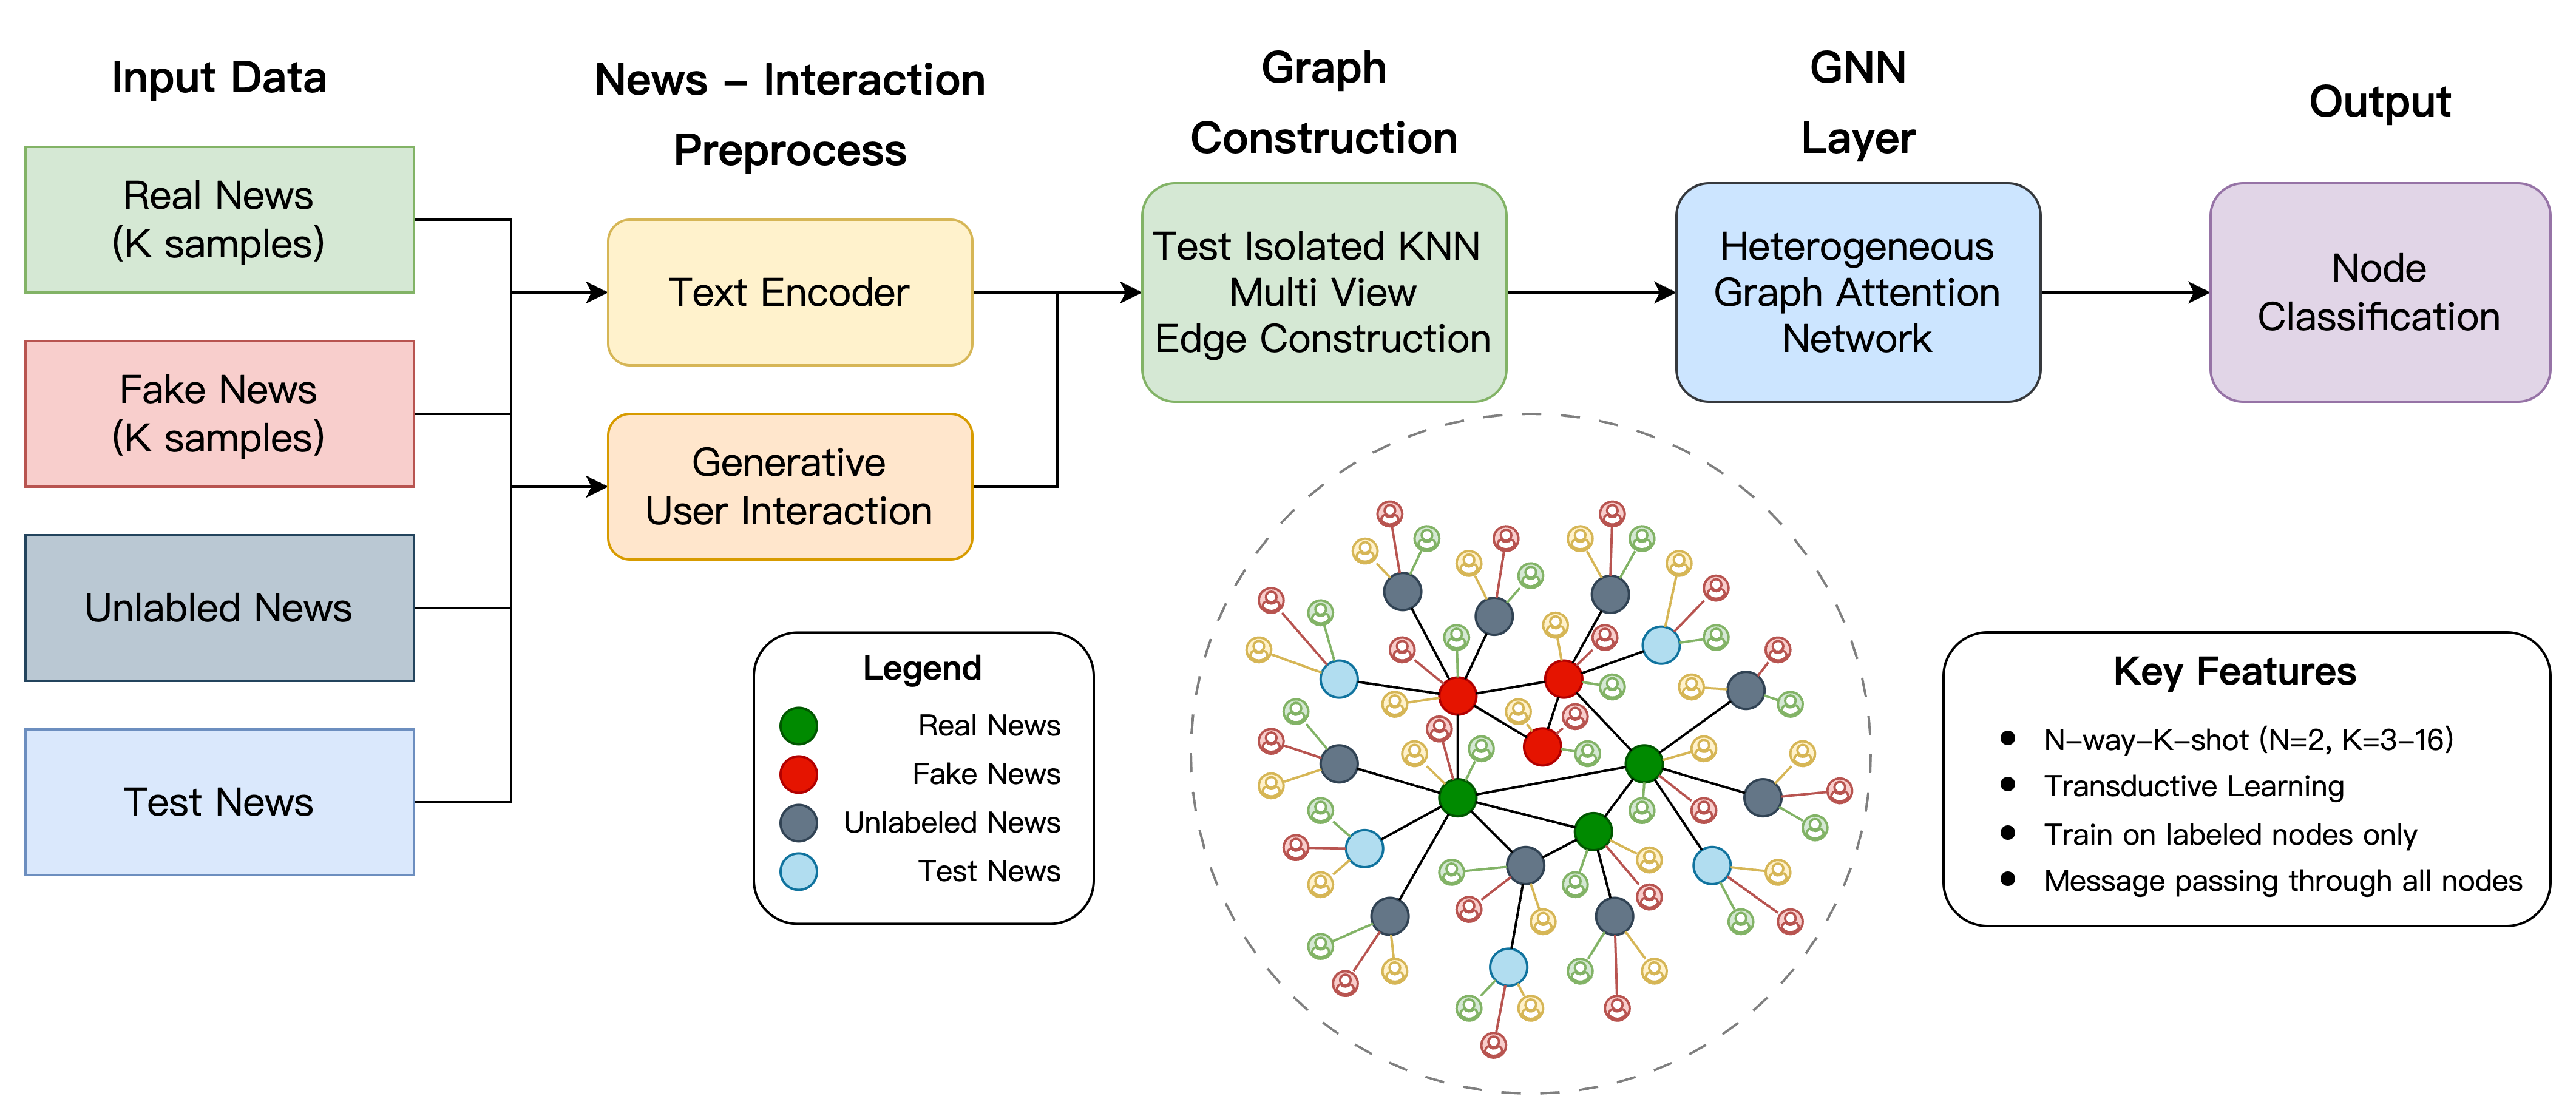
\includegraphics[width=0.8\textwidth]{context/methodology/fig/pipeline.png}
    \caption{Complete GemGNN pipeline showing data flow from news articles through heterogeneous graph construction to final classification}
    \label{fig:pipeline}
\end{figure}

The framework operates under a transductive learning paradigm where all nodes (labeled, unlabeled, and test) participate in heterogeneous message passing, but only labeled nodes contribute to loss computation. This approach maximizes the utility of limited supervision by leveraging the heterogeneous graph structure to propagate information from labeled news nodes to unlabeled and test nodes through learned type-specific attention mechanisms. The choice between traditional KNN and test-isolated KNN allows for flexible adaptation to different deployment scenarios while maintaining consistent architectural principles.

% Comment: The transductive approach is particularly important for few-shot scenarios where every piece of information must be maximally utilized

Our approach begins with pre-trained DeBERTa embeddings for news articles, which provide rich semantic representations (768-dimensional vectors) that capture contextual relationships and linguistic patterns indicative of misinformation. These embeddings serve as the foundation for both similarity-based graph construction and node feature initialization in our heterogeneous graph neural network, ensuring that the model can leverage state-of-the-art natural language understanding capabilities.

The key innovation lies in creating a heterogeneous graph structure that includes both news nodes (representing articles) and interaction nodes (representing synthetic user responses), connected through multiple edge types that capture different semantic relationships. This heterogeneous structure enables the model to learn from both content similarity patterns and social interaction patterns without requiring real user data, addressing privacy constraints while maintaining modeling flexibility.

\section{Generative User Interaction Simulation}

Traditional propagation-based fake news detection methods rely on real user interaction data, which is often unavailable due to privacy constraints or platform limitations. To address this fundamental limitation, we introduce a novel generative approach that synthesizes realistic user interactions using Large Language Models.

\subsection{LLM-based Interaction Generation}

We employ Google's Gemini LLM to generate diverse user interactions for each news article. The generation process is designed to simulate authentic user responses that would naturally occur in social media environments. For each news article $n_i$, we generate a set of user interactions $I_i = \{i_1, i_2, \ldots, i_{20}\}$ where each interaction represents a potential user response to the news content.

The prompt engineering strategy (see Figure~\ref{fig:prompt}) ensures that generated interactions reflect realistic user behavior patterns observed in social media platforms. We incorporate the complete news content, including headlines and article body, to generate contextually appropriate responses that capture various user perspectives and emotional reactions.

\begin{figure}[h]
    \centering
    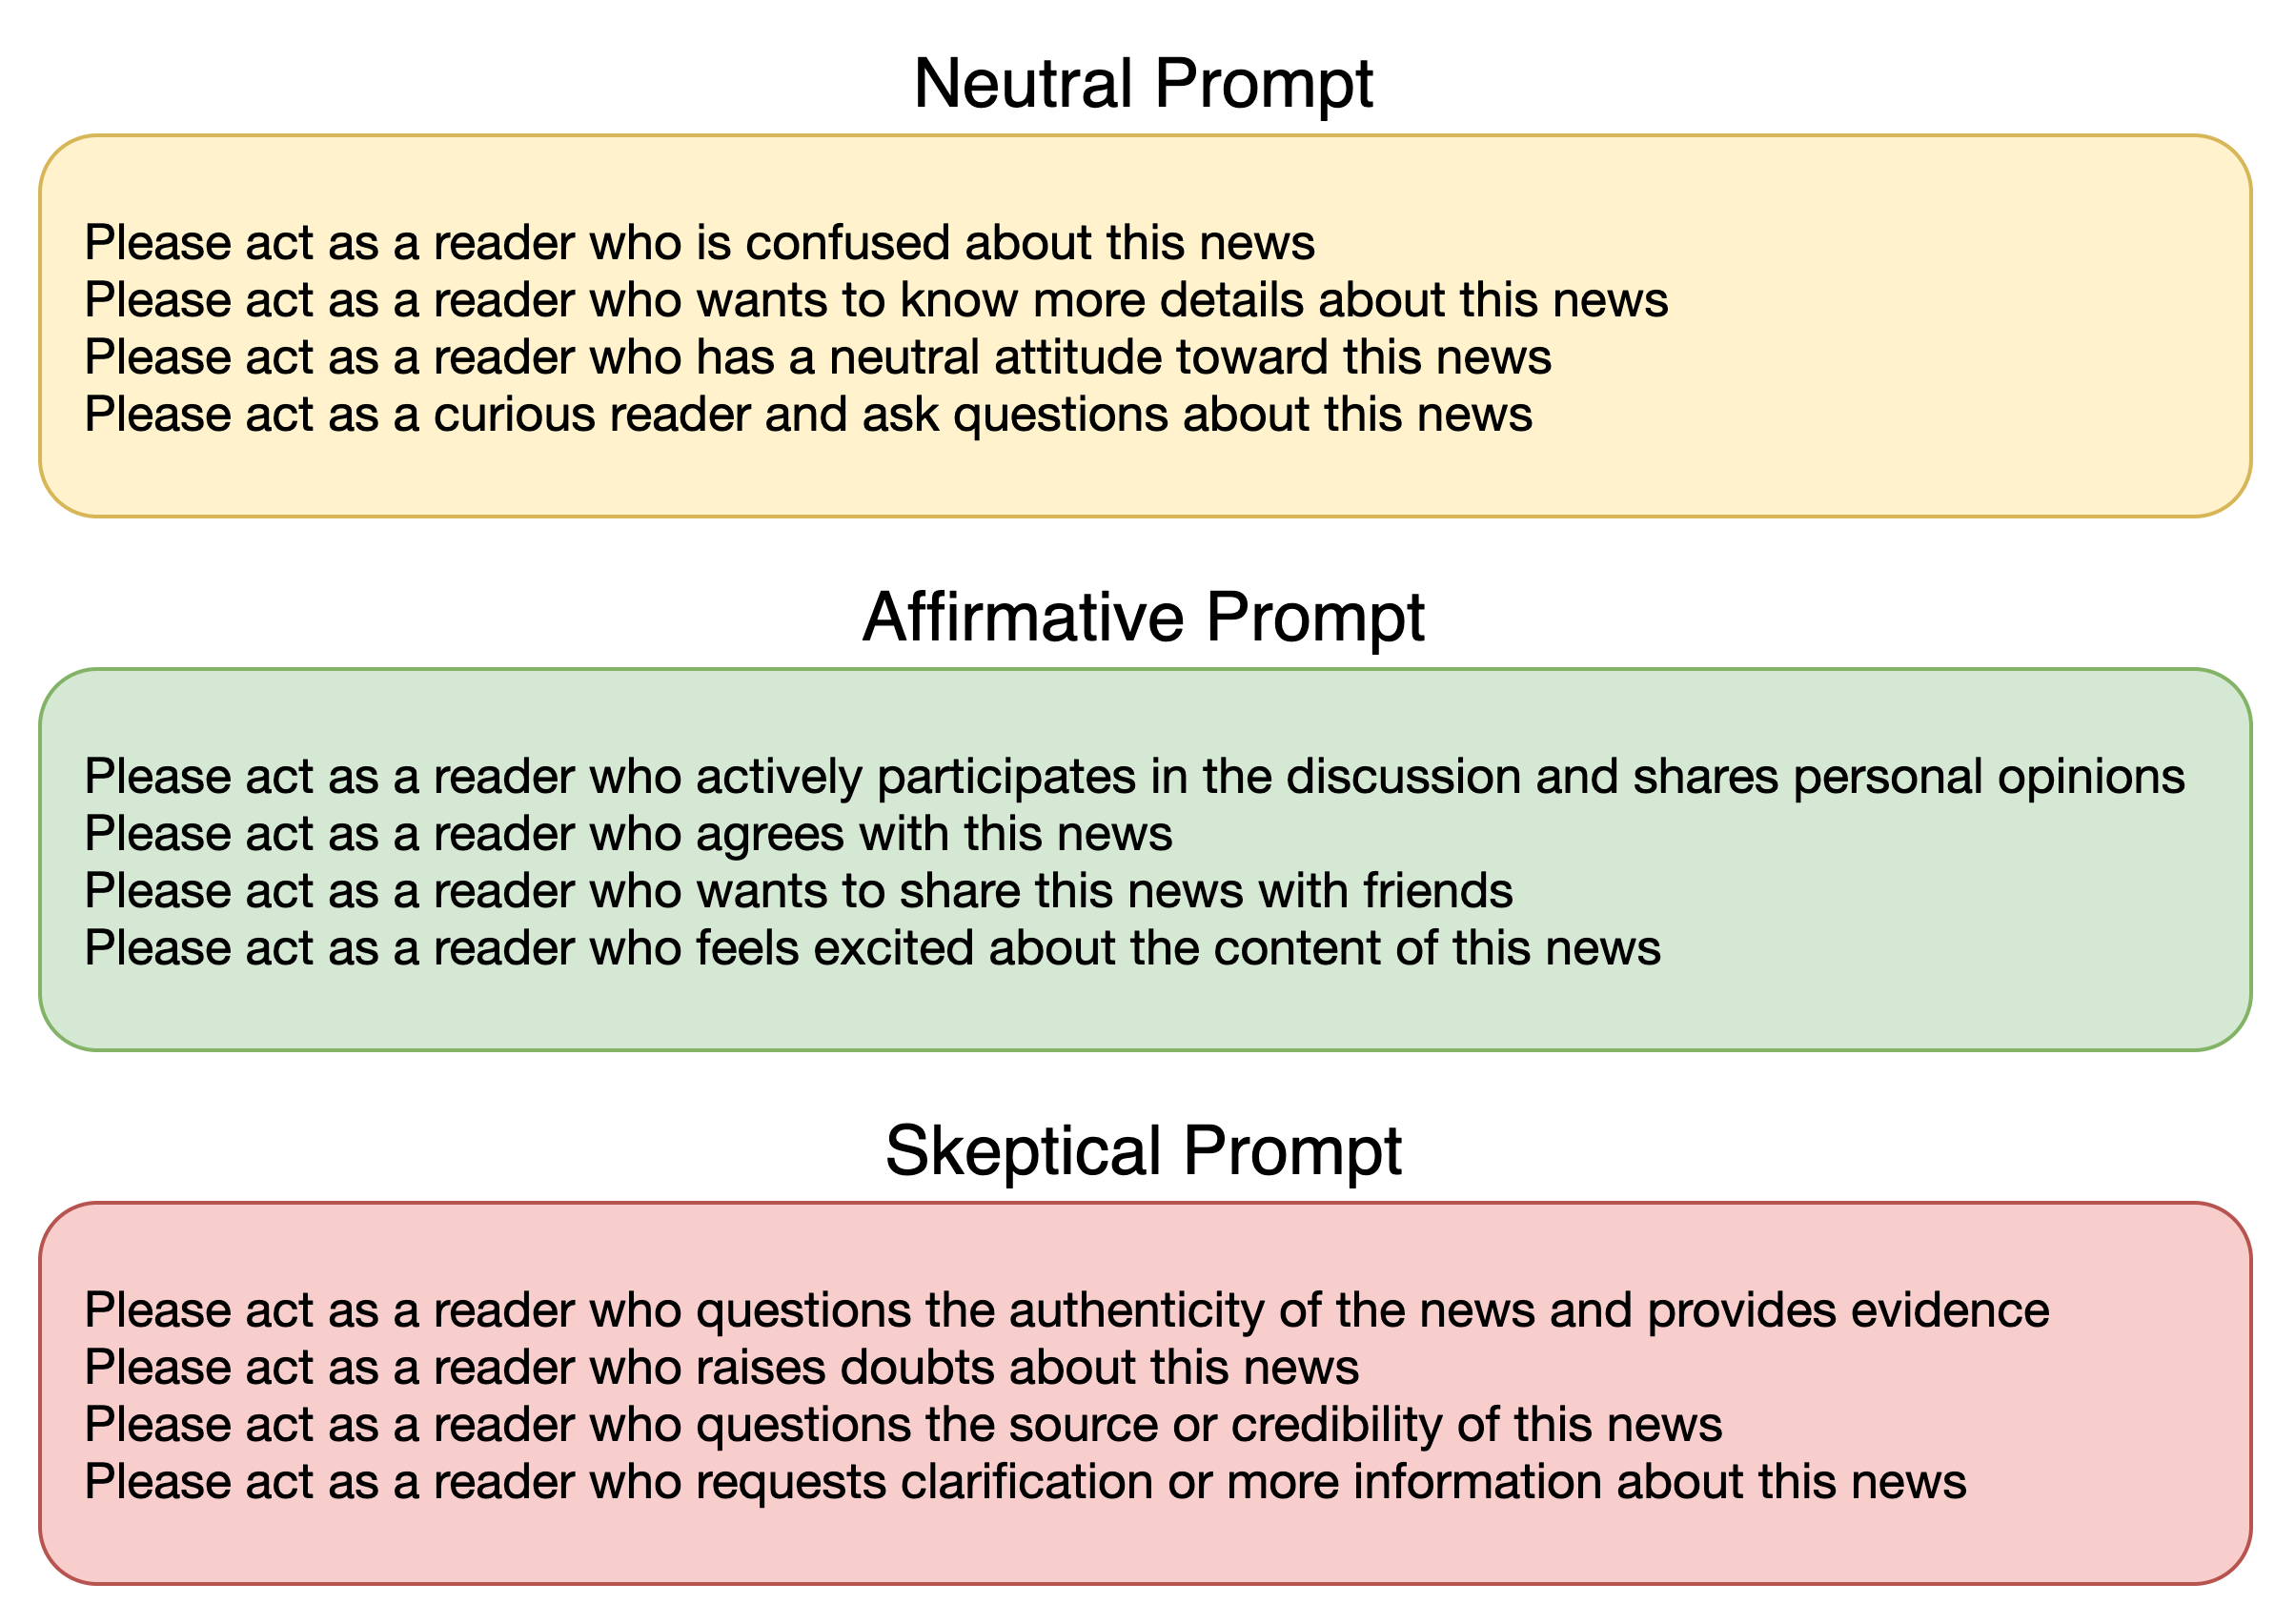
\includegraphics[width=0.5\textwidth]{context/methodology/fig/prompt.png}
    \caption{Prompt engineering strategy}
    \label{fig:prompt}
\end{figure}

\subsection{Multi-tone Interaction Design}

To capture the diversity of user reactions to news content, we implement a structured multi-tone generation strategy (see Figure~\ref{fig:interaction-generation}) with 20 interactions per article that produces interactions across three distinct emotional categories:

\begin{figure}[h]
    \centering
    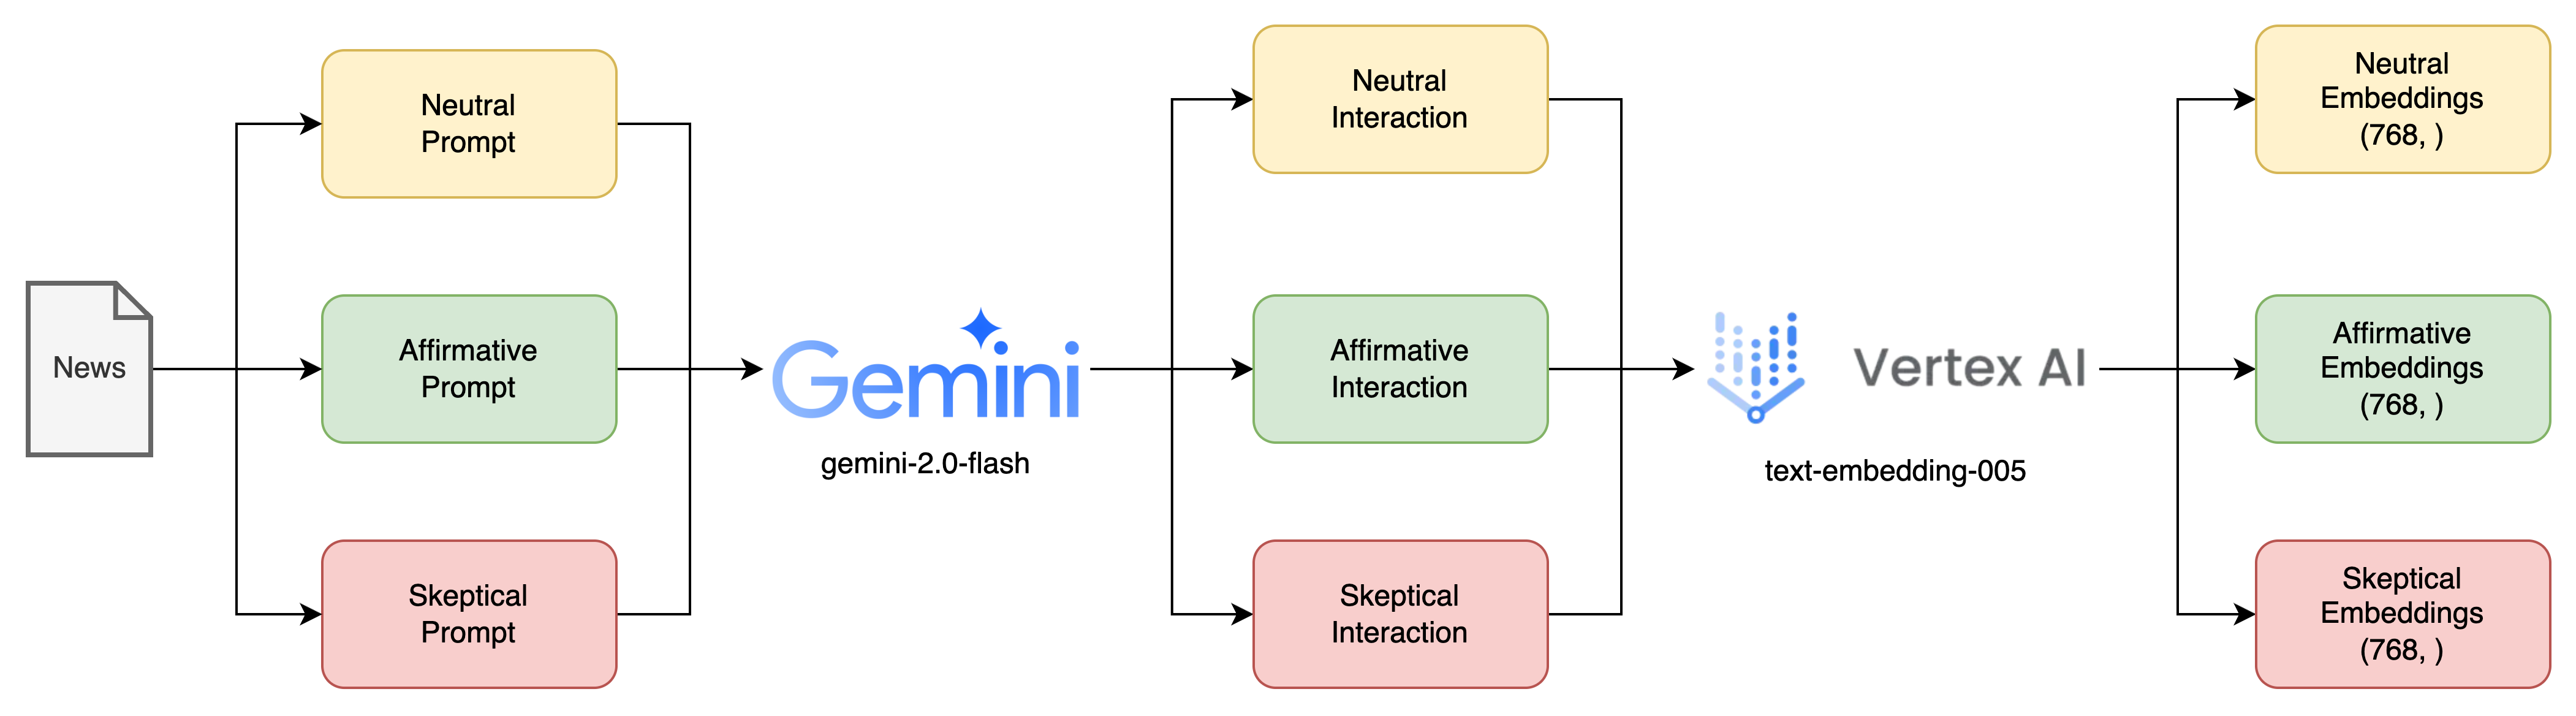
\includegraphics[width=0.8\textwidth]{context/methodology/fig/user_interaction_generation.png}
    \caption{Multi-tone interaction generation strategy}
    \label{fig:interaction-generation}
\end{figure}

\textbf{Neutral Interactions (8 per article):} These represent objective, factual responses that focus on information sharing without emotional bias. Neutral interactions typically include questions for clarification, requests for additional sources, or straightforward restatements of key facts.

\textbf{Affirmative Interactions (7 per article):} These capture supportive or agreeable responses from users who accept the news content as credible. Affirmative interactions include expressions of agreement, sharing intentions, and positive emotional responses.

\textbf{Skeptical Interactions (5 per article):} These represent critical or questioning responses from users who doubt the veracity of the news content. Skeptical interactions include challenges to facts, requests for verification, and expressions of disbelief or concern.

This distribution (8:7:5) reflects observed patterns in real social media interactions where neutral responses predominate, followed by supportive reactions, with skeptical responses being less common but highly informative for authenticity assessment.

\subsection{Interaction-News Edge Construction}

Each generated interaction is embedded using the VertexAI text-embedding-005 model. The interactions are connected to their corresponding news articles through directed edges that carry tone information as edge attributes (see Figure~\ref{fig:news_interaction_node}).

\begin{figure}[h]
    \centering
    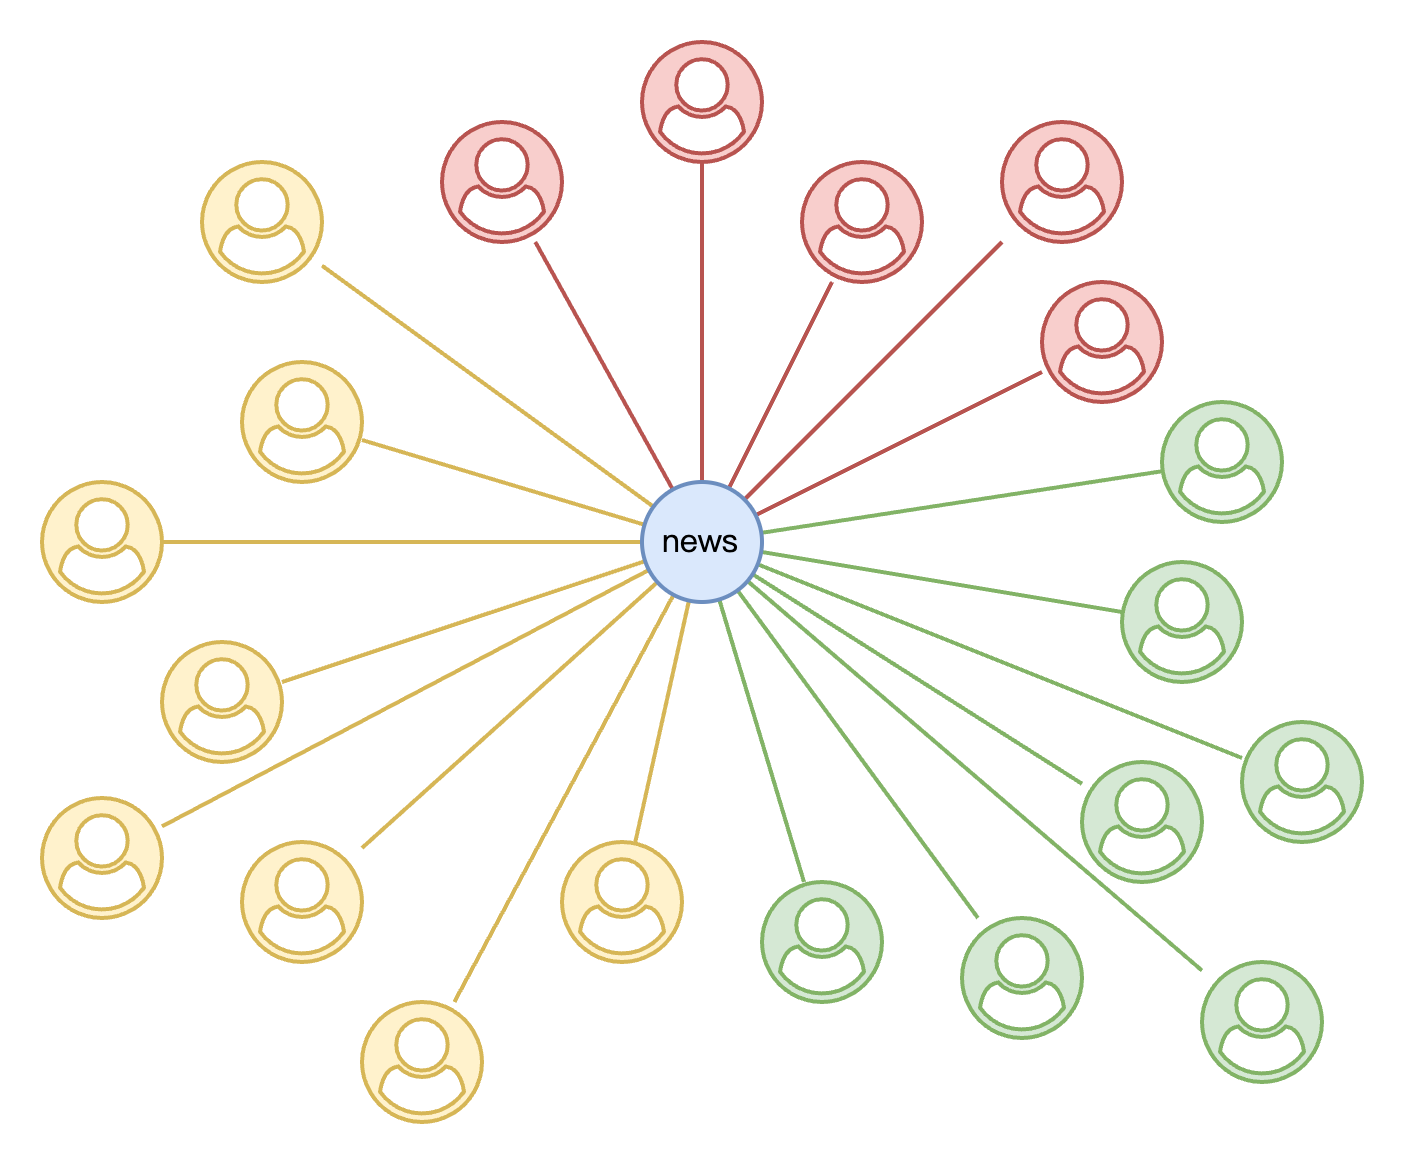
\includegraphics[width=0.5\textwidth]{context/methodology/fig/news_interaction_node.png}
    \caption{Interaction-News edge construction}
    \label{fig:news_interaction_node}
\end{figure}

Formally, for each news article $n_i$ and its generated interactions $I_i$, we create edges $(n_i, i_j)$ where the edge attribute $a_{ij}$ encodes the interaction tone: $a_{ij} \in \{0, 1, 2\}$ representing neutral, affirmative, and skeptical tones respectively. This encoding allows the heterogeneous graph attention network to learn tone-specific importance weights during message aggregation.

\section{Graph Construction Methodologies: KNN vs Test-Isolated KNN}

Graph edge construction is a fundamental design choice that significantly impacts both model performance and evaluation realism in few-shot fake news detection. We explore two complementary approaches: traditional KNN and Test-Isolated KNN (see Figure~\ref{fig:edge_construction}), each suited to different real-world deployment scenarios and research objectives. Our experimental analysis reveals that these approaches offer distinct trade-offs between performance optimization and evaluation integrity, necessitating careful consideration of the intended application context.

\begin{figure}[h]
    \centering
    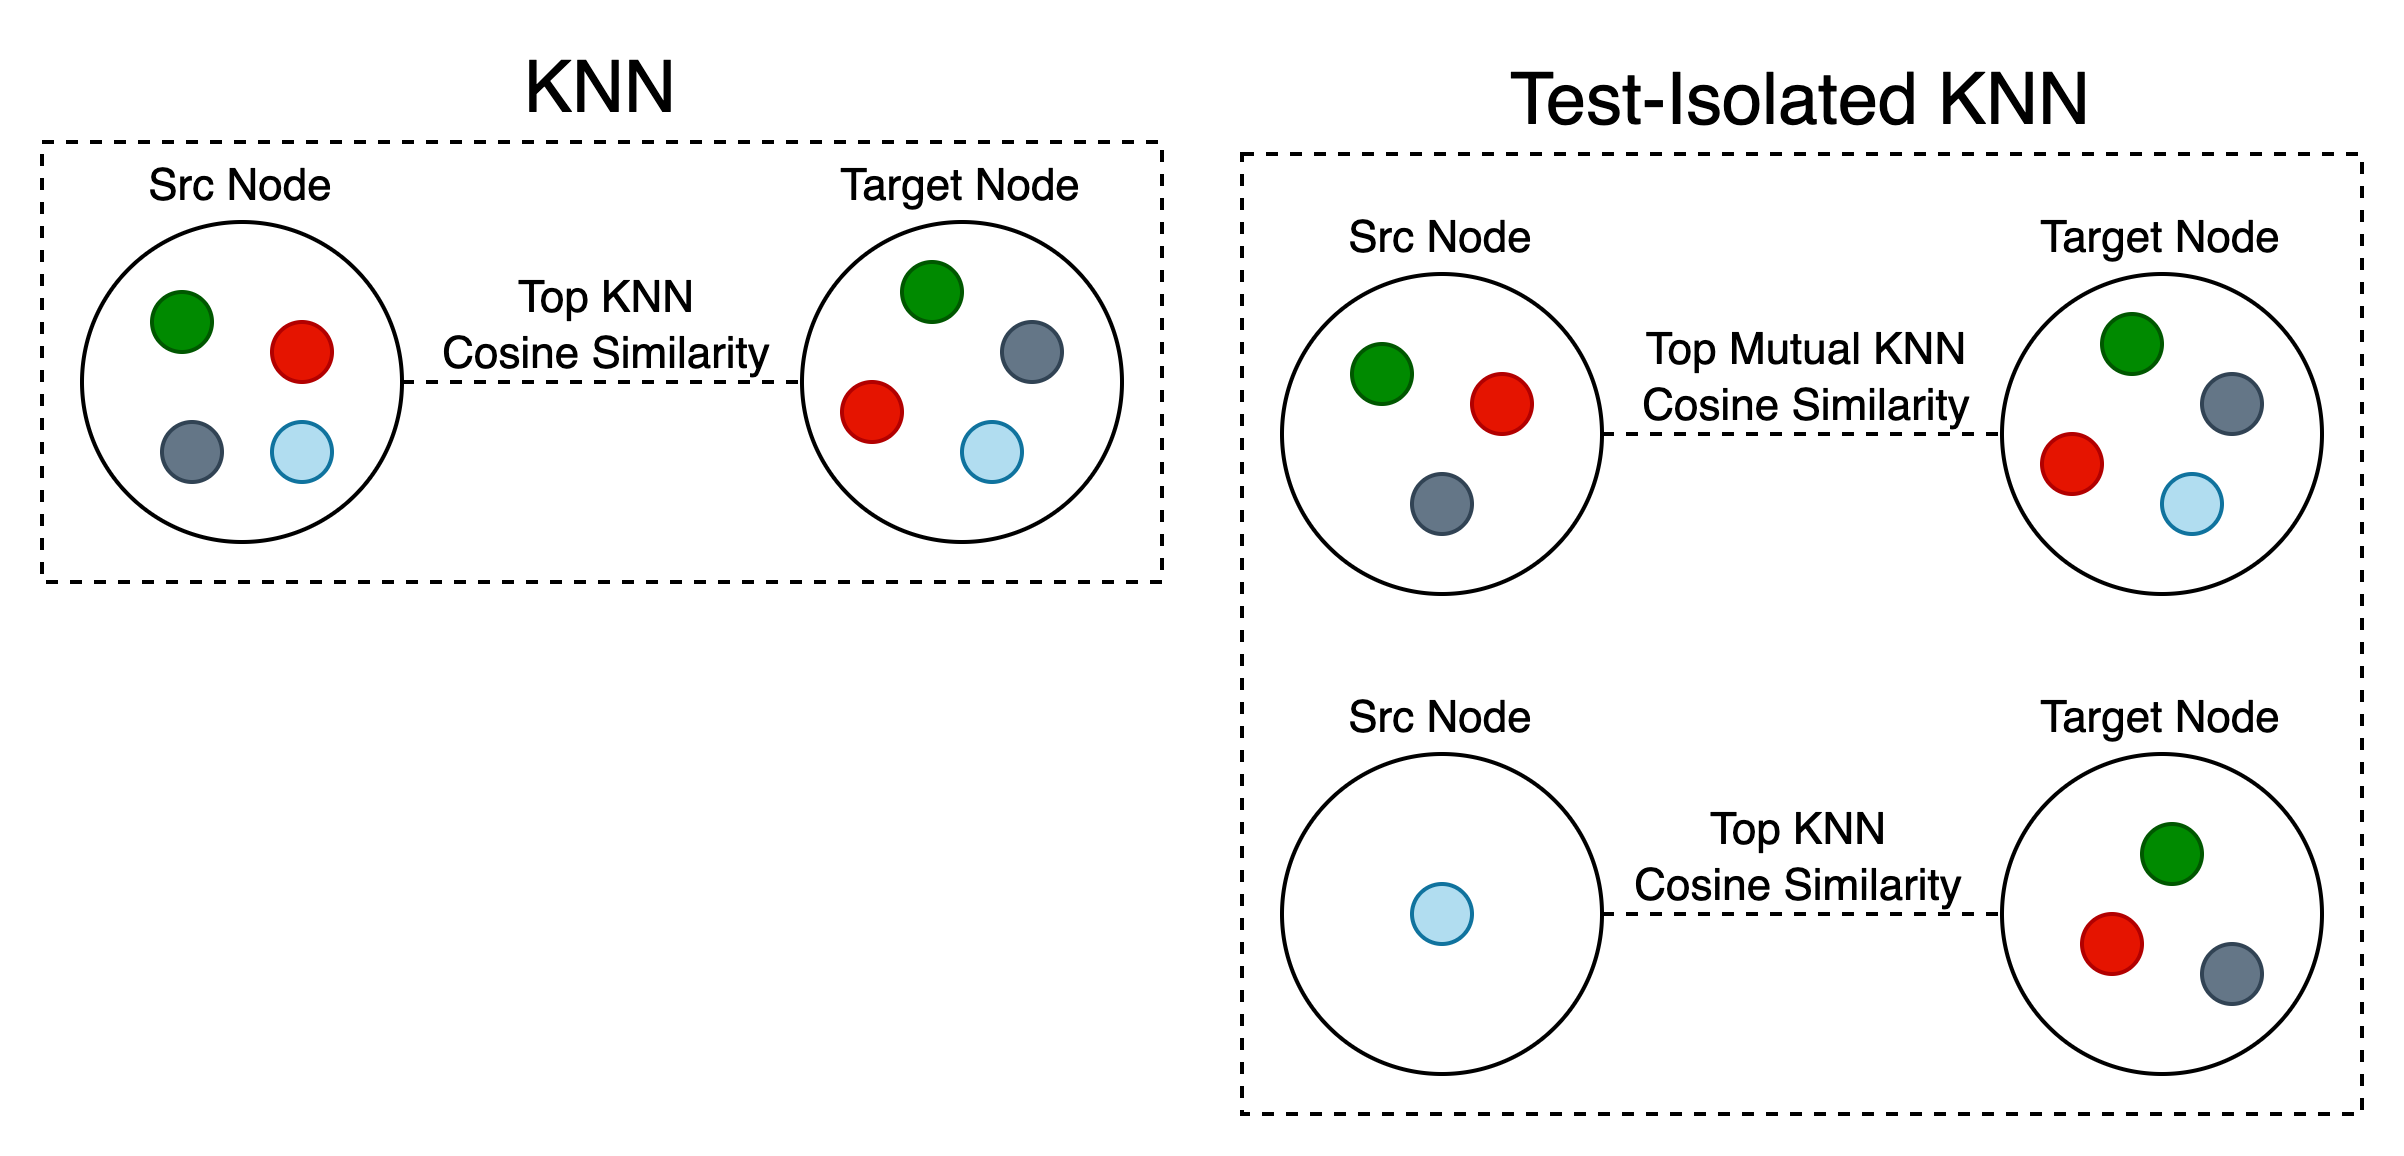
\includegraphics[width=0.5\textwidth]{context/methodology/fig/edge_construction.png}
    \caption{Traditional KNN vs Test-Isolated KNN}
    \label{fig:edge_construction}
\end{figure}

\subsection{Traditional KNN: Performance-Optimized Graph Construction}

Traditional K-Nearest Neighbor (KNN) graph construction allows all nodes, including test instances, to connect to their most similar neighbors regardless of their dataset partition. This approach maximizes information flow throughout the graph, enabling comprehensive message passing that can improve classification performance.

\textbf{Methodology:} For each node $n_i$ in the dataset (training, validation, or test), we compute pairwise cosine similarities with all other nodes using DeBERTa embeddings and establish edges to the top-$k$ most similar instances. This creates a densely connected graph where test nodes can potentially connect to other test nodes, labeled training samples, and unlabeled instances.

\textbf{Real-World Applicability:} Traditional KNN is particularly suitable for \emph{batch processing scenarios} where multiple news articles arrive simultaneously and can be processed collectively. Examples include:
\begin{itemize}
    \item Daily fact-checking workflows where news articles from the same time period are analyzed together
    \item Retrospective analysis of misinformation campaigns where temporal constraints are relaxed
    \item Content moderation systems that process articles in batches rather than real-time streams
    \item Research environments where maximizing detection accuracy is prioritized over strict temporal realism
\end{itemize}

In these scenarios, the assumption that articles can share information during inference is reasonable, as human fact-checkers often cross-reference multiple articles and consider contextual relationships when making verification decisions.

\subsection{Test-Isolated KNN: Evaluation-Realistic Graph Construction}

Test-Isolated KNN enforces strict separation between test instances, prohibiting direct connections between test nodes while maintaining connectivity to training data. This approach prioritizes evaluation realism over raw performance, ensuring that model assessment reflects realistic deployment conditions.

\textbf{Methodology:} Test nodes are restricted to connect only to training nodes (labeled and unlabeled), while training nodes can connect to any other training nodes through mutual KNN relationships. For each test node $n_{test}$, we identify the top-$k$ most similar training instances and create unidirectional edges from training to test nodes.

\textbf{Real-World Applicability:} Test-isolated KNN is essential for \emph{streaming deployment scenarios} where news articles arrive independently and must be classified without knowledge of future instances. Examples include:
\begin{itemize}
    \item Real-time social media monitoring where articles appear sequentially
    \item Breaking news verification systems with strict temporal constraints
    \item Production deployments where test instances represent genuinely unknown future data
    \item Academic evaluation protocols that prioritize methodological rigor and reproducibility
\end{itemize}

This approach ensures that performance estimates accurately reflect the model's ability to generalize to truly unseen data, preventing artificially inflated results from test-test information sharing.

\subsection{Performance vs. Realism Trade-off Analysis}

Our comprehensive experimental evaluation across GossipCop and PolitiFact datasets reveals consistent patterns in the performance trade-offs between these approaches:

\textbf{GossipCop Results:}
\begin{itemize}
    \item Traditional KNN: Average F1 = 0.5849
    \item Test-Isolated KNN: Average F1 = 0.5738
    \item Performance difference: 1.9\% decrease with test isolation
\end{itemize}

\textbf{PolitiFact Results:}
\begin{itemize}
    \item Traditional KNN: Average F1 = 0.7815
    \item Test-Isolated KNN: Average F1 = 0.7756
    \item Performance difference: 0.8\% decrease with test isolation
\end{itemize}

These results demonstrate that test isolation imposes a modest but consistent performance penalty while providing more realistic evaluation conditions. The trade-off magnitude varies by dataset characteristics, with more complex datasets (GossipCop) showing larger performance gaps.

\subsection{Deployment Context Decision Framework}

The choice between KNN approaches should be guided by specific deployment requirements and evaluation objectives:

\textbf{Choose Traditional KNN when:}
\begin{itemize}
    \item Maximizing detection accuracy is the primary objective
    \item Articles are processed in batches where cross-referencing is acceptable
    \item Historical analysis or retrospective fact-checking scenarios
    \item Sufficient computational resources allow comprehensive similarity analysis
\end{itemize}

\textbf{Choose Test-Isolated KNN when:}
\begin{itemize}
    \item Realistic evaluation and fair model comparison are critical
    \item Simulating real-time or streaming deployment conditions
    \item Academic research requiring methodological rigor
    \item Production systems where test instances represent genuinely unknown future data
\end{itemize}

\textbf{Hybrid Approaches:} For complex production systems, a hybrid strategy may be optimal, using traditional KNN for training and validation while employing test-isolated evaluation protocols to ensure realistic performance estimates.

\subsection{Technical Implementation Details}

\textbf{Mutual KNN for Training Nodes:} In both approaches, training nodes (labeled and unlabeled) employ mutual KNN connections to ensure robust semantic relationships. Given the set of training nodes $N_{train} = N_{labeled} \cup N_{unlabeled}$, we compute pairwise cosine similarities between DeBERTa embeddings and select the top-$k$ nearest neighbors for each node.

The mutual KNN constraint ensures that if node $n_i$ selects $n_j$ as a neighbor, then $n_j$ must also select $n_i$ among its top-$k$ neighbors. This bidirectionality strengthens connections between truly similar articles while reducing noise from asymmetric similarity relationships.

\textbf{Test Node Connectivity Strategies:}
\begin{itemize}
    \item \textbf{Traditional KNN:} Test nodes can connect to their top-$k$ similar nodes from any partition (training, validation, or test), enabling maximum information flow.
    \item \textbf{Test-Isolated KNN:} Test nodes connect only to their top-$k$ most similar training instances through unidirectional edges, maintaining evaluation integrity.
\end{itemize}

The choice of connectivity strategy directly impacts both the information available during message passing and the realism of the evaluation protocol, highlighting the importance of aligning methodology with intended application context.

\section{DeBERTa vs RoBERTa: Text Encoder Selection Rationale}

The choice of text encoder fundamentally impacts both the quality of initial node representations and the effectiveness of multi-view graph construction. We adopt DeBERTa (Decoding-enhanced BERT with Disentangled Attention) over RoBERTa based on its superior characteristics for embedding partitioning and multi-view learning.

\subsection{Disentangled Attention and Embedding Structure}

DeBERTa's key innovation lies in its disentangled attention mechanism, which separates content and position representations throughout the transformer layers. This architectural design creates embeddings with more structured internal organization compared to RoBERTa's standard attention mechanism.

\textbf{Content-Position Separation:} DeBERTa computes attention weights using separate representations for content and relative position information, leading to embeddings where different dimensions capture distinct semantic aspects more cleanly. This separation is crucial for our multi-view approach, which relies on partitioning embeddings into coherent semantic subspaces.

\textbf{Enhanced Relative Position Encoding:} DeBERTa's improved relative position encoding creates embeddings that better preserve syntactic and discourse-level information across different dimensional ranges, making the embeddings more amenable to meaningful partitioning.

\subsection{Multi-View Embedding Partitioning Advantages}

The structured nature of DeBERTa embeddings provides several advantages for multi-view graph construction:

\textbf{Semantic Coherence Preservation:} When DeBERTa embeddings are partitioned into subsets (e.g., $\mathbf{h}_i^{(1)}, \mathbf{h}_i^{(2)}, \mathbf{h}_i^{(3)} \in \mathbb{R}^{256}$), each partition retains meaningful semantic information rather than becoming arbitrary dimensional slices. This is because DeBERTa's disentangled attention naturally organizes embedding dimensions according to different linguistic aspects.

\textbf{Complementary View Construction:} The architectural separation in DeBERTa enables more effective partitioning strategies:
\begin{itemize}
    \item \textbf{Early dimensions} (view 1): Capture syntactic patterns and surface-level linguistic features
    \item \textbf{Middle dimensions} (view 2): Represent semantic relationships and contextual dependencies  
    \item \textbf{Later dimensions} (view 3): Encode higher-level discourse and pragmatic information
\end{itemize}

\textbf{Information Retention Under Partitioning:} Unlike RoBERTa embeddings, which may lose critical information when partitioned due to their more entangled representation structure, DeBERTa embeddings maintain sufficient discriminative power even when split into smaller subsets. This property is essential for our multi-view approach to remain effective.

\subsection{Empirical Validation of Encoder Choice}

Our preliminary experiments comparing DeBERTa and RoBERTa for multi-view graph construction demonstrate clear advantages:

\textbf{Partition Quality Analysis:} DeBERTa partitions show higher within-view coherence and between-view diversity, measured through semantic similarity metrics and clustering analysis. Each DeBERTa partition captures distinct aspects of news content, while RoBERTa partitions exhibit more overlap and redundancy.

\textbf{Multi-View Performance:} The multi-view approach with DeBERTa consistently outperforms single-view baselines by larger margins compared to RoBERTa-based multi-view implementations, indicating more effective utilization of the partitioned representations.

\textbf{Robustness to Partitioning:} DeBERTa embeddings maintain stable performance across different partitioning strategies and view counts, while RoBERTa shows higher sensitivity to partition configuration, suggesting less organized internal structure.

\subsection{Computational and Practical Considerations}

\textbf{Model Size and Efficiency:} While DeBERTa-base has similar computational requirements to RoBERTa-base (110M vs 125M parameters), its superior partitioning properties justify the choice for multi-view architectures where embedding quality is paramount.

\textbf{Pre-training Alignment:} DeBERTa's pre-training objectives and architectural design align well with fake news detection tasks, which require understanding of subtle linguistic cues, discourse patterns, and contextual relationships that benefit from disentangled representations.

This encoder selection provides the foundation for effective multi-view graph construction, where the quality of embedding partitions directly impacts the diversity and effectiveness of different semantic perspectives captured in our heterogeneous graph architecture.

\section{Multi-View Graph Construction}

To capture diverse semantic perspectives within news content, we implement a multi-view learning framework (see Figure~\ref{fig:multi_view}) that partitions embeddings into complementary views and constructs separate graph structures for each perspective.

\begin{figure}[h]
    \centering
    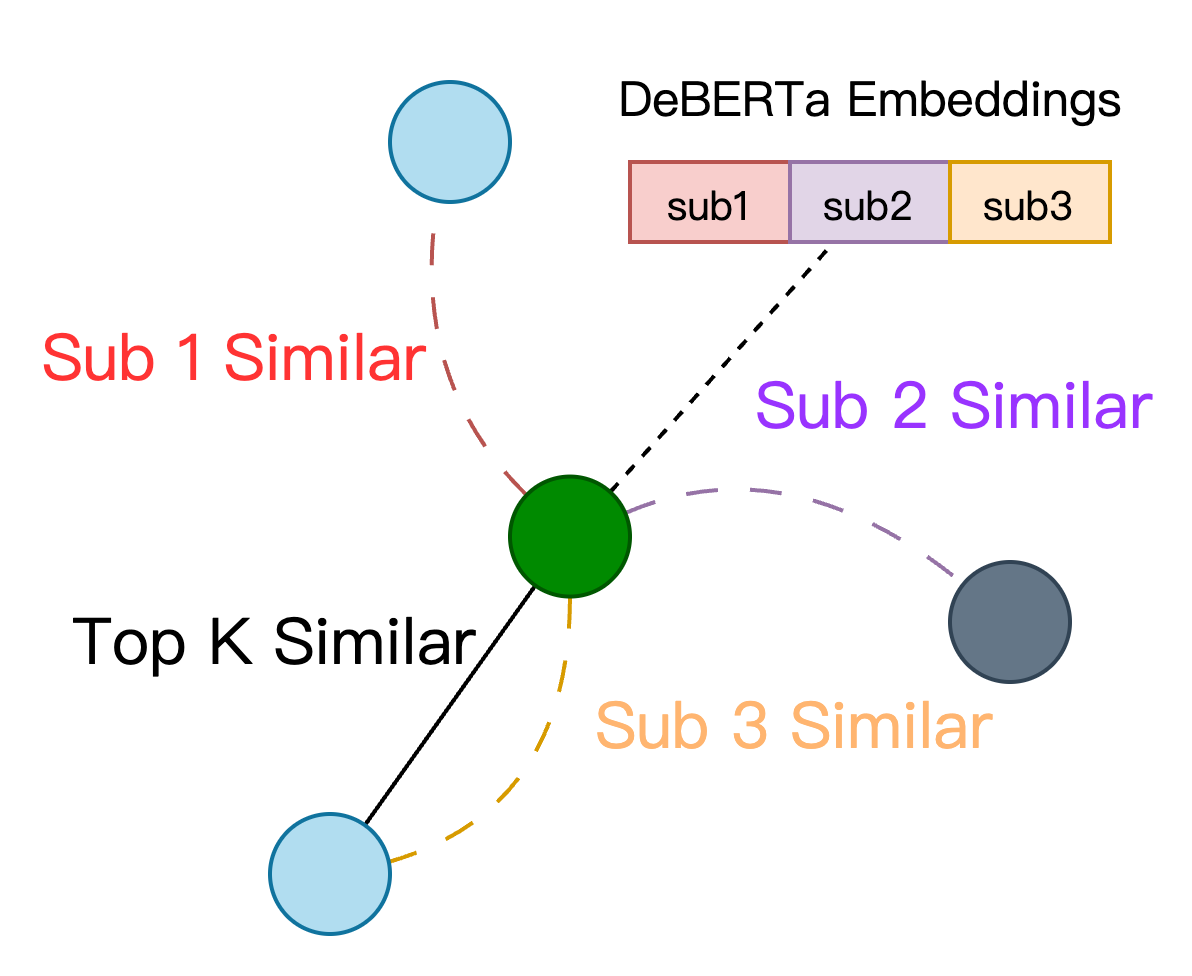
\includegraphics[width=0.5\textwidth]{context/methodology/fig/multi_view.png}
    \caption{Utilizing DeBERTa's disentangled attention architecture to partition embeddings into complementary views}
    \label{fig:multi_view}
\end{figure}

\subsection{Embedding Dimension Splitting Strategy}

Given DeBERTa embeddings of dimension $d = 768$, we partition each embedding vector into three equal subsets: $\mathbf{h}_i^{(1)}, \mathbf{h}_i^{(2)}, \mathbf{h}_i^{(3)} \in \mathbb{R}^{256}$ where $\mathbf{h}_i = [\mathbf{h}_i^{(1)}; \mathbf{h}_i^{(2)}; \mathbf{h}_i^{(3)}]$.

This partitioning strategy is fundamentally enabled by DeBERTa's disentangled attention architecture, which creates natural organization within embedding dimensions. Each view captures different aspects of the semantic representation:

\textbf{View 1 (Dimensions 0-255):} Focuses on early embedding dimensions that typically encode syntactic patterns, surface-level linguistic features, and basic semantic relationships. These dimensions capture immediate lexical signals and structural patterns that are crucial for initial content assessment.

\textbf{View 2 (Dimensions 256-511):} Captures semantic relationships, contextual dependencies, and mid-level discourse patterns. This middle partition leverages DeBERTa's enhanced position encoding to represent contextual relationships and thematic coherence.

\textbf{View 3 (Dimensions 512-767):} Represents higher-level abstractions, discourse-level information, and pragmatic content understanding. These later dimensions encode sophisticated linguistic patterns and meta-textual features that are particularly important for detecting subtle misinformation cues.

The effectiveness of this partitioning relies on DeBERTa's structured representation organization, where the disentangled attention mechanism ensures that different dimensional ranges capture complementary rather than redundant information aspects.

\subsection{View-specific Edge Construction}

For each view $v \in \{1, 2, 3\}$, we apply the chosen graph construction strategy (traditional KNN or test-isolated KNN) using view-specific embeddings $\mathbf{h}_i^{(v)}$. This process generates three distinct graph structures $G^{(1)}, G^{(2)}, G^{(3)}$ where each graph emphasizes different semantic relationships between news articles.

The choice of edge construction strategy (KNN vs test-isolated KNN) is maintained consistently across all views to ensure methodological coherence. The diversity of edge connections across views ensures that the model learns to integrate multiple perspectives of similarity, forcing it to develop more robust and generalizable feature representations. Articles that appear similar in one semantic view may differ significantly in another, providing complementary information for classification.

\subsection{Multi-Graph Training Strategy}

During training, we process all three views simultaneously, computing separate message passing operations for each graph structure. The view-specific representations are combined through learned attention mechanisms that dynamically weight the importance of each perspective based on the classification task.

This multi-graph approach serves as a form of data augmentation at the graph level, exposing the model to varied structural contexts that improve robustness and generalization. The diverse connectivity patterns help prevent overfitting to specific graph topologies and enhance the model's ability to handle different types of news content.

\section{Heterogeneous Graph Architecture}

\subsection{Node Types and Features}

Our heterogeneous graph contains two primary node types:

\textbf{News Nodes:} Represent news articles with DeBERTa embeddings as node features. Each news node $n_i$ has features $\mathbf{x}_i \in \mathbb{R}^{768}$ and a binary label $y_i \in \{0, 1\}$ indicating real (0) or fake (1) news for labeled instances.

\textbf{Interaction Nodes:} Represent generated user interactions with DeBERTa embeddings as features. Each interaction node $i_j$ has features $\mathbf{x}_j \in \mathbb{R}^{768}$ and is connected to exactly one news article through tone-specific edges.

\subsection{Edge Types and Relations}

The heterogeneous graph incorporates multiple edge types that capture different relationship semantics:

\textbf{News-to-News Edges:} Connect semantically similar news articles based on the chosen graph construction strategy (traditional KNN or test-isolated KNN). These edges enable direct information flow between related news content and are the primary mechanism for few-shot learning.

\textbf{News-to-Interaction Edges:} Connect news articles to their generated user interactions, with edge attributes encoding interaction tones. These edges allow the model to incorporate user perspective information into news classification.

\textbf{Interaction-to-News Edges:} Reverse connections that enable bidirectional information flow between news content and user reactions, allowing interaction patterns to influence news representations.

\subsection{HAN-based Message Passing and Classification}

We employ Heterogeneous Graph Attention Networks (HAN) as our base architecture due to their ability to handle multiple node and edge types through specialized attention mechanisms. The HAN architecture consists of two levels of attention: node-level attention and semantic-level attention.

\textbf{Node-level Attention:} For each edge type, we compute attention weights between connected nodes:
\begin{equation}
\alpha_{ij}^{\phi} = \frac{\exp(\sigma(\mathbf{a}_{\phi}^T[\mathbf{W}_{\phi}\mathbf{h}_i \| \mathbf{W}_{\phi}\mathbf{h}_j]))}{\sum_{k \in \mathcal{N}_i^{\phi}} \exp(\sigma(\mathbf{a}_{\phi}^T[\mathbf{W}_{\phi}\mathbf{h}_i \| \mathbf{W}_{\phi}\mathbf{h}_k]))}
\end{equation}

where $\phi$ represents the edge type, $\mathbf{W}_{\phi}$ is the edge-type-specific transformation matrix, and $\mathbf{a}_{\phi}$ is the attention vector.

\textbf{Semantic-level Attention:} We aggregate information across different edge types using learned importance weights:
\begin{equation}
\beta_{\phi} = \frac{1}{|\mathcal{V}|} \sum_{i \in \mathcal{V}} q^T \tanh(\mathbf{W} \cdot \mathbf{h}_i^{\phi} + \mathbf{b})
\end{equation}

where $\mathbf{h}_i^{\phi}$ is the node representation for edge type $\phi$, and $q$, $\mathbf{W}$, $\mathbf{b}$ are learnable parameters.

The final node representation combines information from all edge types:
\begin{equation}
\mathbf{h}_i = \sum_{\phi \in \Phi} \beta_{\phi} \mathbf{h}_i^{\phi}
\end{equation}

\section{Loss Function Design and Training Strategy}

\subsection{Enhanced Loss Functions for Few-Shot Learning}

To address the challenges of few-shot learning, we implement enhanced loss functions that incorporate label smoothing and focal loss components to improve model robustness and handle class imbalance effectively.

\textbf{Label Smoothing Cross-Entropy:} We apply label smoothing with parameter $\epsilon = 0.1$ to prevent overconfident predictions on limited training data:
\begin{equation}
\mathcal{L}_{smooth} = -\sum_{i=1}^{N} \sum_{c=1}^{C} y_i^{smooth}(c) \log p_i(c)
\end{equation}

where $y_i^{smooth}(c) = (1-\epsilon)y_i(c) + \frac{\epsilon}{C}$ and $p_i(c)$ is the predicted probability for class $c$.

\textbf{Focal Loss Component:} To address potential class imbalance, we incorporate a focal loss term that down-weights easy examples and focuses learning on difficult instances:
\begin{equation}
\mathcal{L}_{focal} = -\alpha \sum_{i=1}^{N} (1-p_i)^{\gamma} \log p_i
\end{equation}

where $\alpha = 0.25$ and $\gamma = 2.0$ are hyperparameters that control the focusing strength.

\subsection{Transductive Learning Framework}

Our training strategy follows a transductive learning paradigm where all nodes participate in message passing, but only labeled nodes contribute to the loss computation. This approach maximizes the utility of unlabeled data by allowing the model to learn better feature representations through graph structure exploration.

The complete loss function combines the enhanced components:
\begin{equation}
\mathcal{L}_{total} = \mathcal{L}_{smooth} + \lambda \mathcal{L}_{focal}
\end{equation}

where $\lambda = 0.1$ balances the contribution of the focal loss component.

Training proceeds for a maximum of 300 epochs with early stopping based on validation performance. We employ the Adam optimizer with learning rate $5 \times 10^{-4}$ and weight decay $1 \times 10^{-3}$ to prevent overfitting in few-shot scenarios.

% ------------------------------------------------
\EndChapter
% ------------------------------------------------